%!TEX root = ../dissertation.tex

\chapter{Introduction}
\label{chapter:introduction}

\section{Motivation}

It has been robotic's long term goal and also, dream, to
have \glspl{SMR} and in particular \glspl{DSR} that can assist humans in
their daily domestic tasks.
This area is a subfield of social robotics which will likely have a considerable
impact on society, not only by improving people's psychological and physical
state, but also by giving them spare time which can be spent doing other
activities. This includes robots: assisting senior citizens
on tasks they can no longer execute on their own (like cooking,
cleaning or organizing medical pills, for example); carrying out tasks for
people with disabilities; and helping or dealing with house chores that are too
cumbersome or repetitive for people. \par

Fortunately, this research area has been pushed forward by recent developments
in machine learning or more generally artificial intelligence. This includes
humongous developments on robot's skills like computer vision, mobile base
navigation, environment mapping, speech processing and recognition, robotic
manipulation and also, human robot interaction.
\par

This momentum on robotics research has so far introduced multiple tools for
roboticists: in software with the introduction of \gls{ROS}\footnote{To know more, check:
\url{http://www.ros.org/}}, and in hardware as stable consumer grade robot
platforms become available from mainstream companies. In turn, public awareness
and interest is increasing with the rise of robotics competitions.
A prime example is Robocup\footnote{For more information see
\url{http://www.robocup.org/}}, the major international robotics competition,
fostering \gls{AI} and robotics research. Its role is to provide
standardized testing environments and tasks in order to properly benchmark
developed technologies by researchers all over the world. All of this while
encouraging healthy competitions and sharing of knowledge between these
international teams.
Therefore, as these areas improve, the goal of having a \gls{GPSR}\footnote{
This is also a name for a specific task in Robocup. Its purpose is to evaluate
how all the different robot skills perform together on a set of possible benchmarks.} 
becomes imminent. 
\par

\begin{figure}[H]
    \centering
        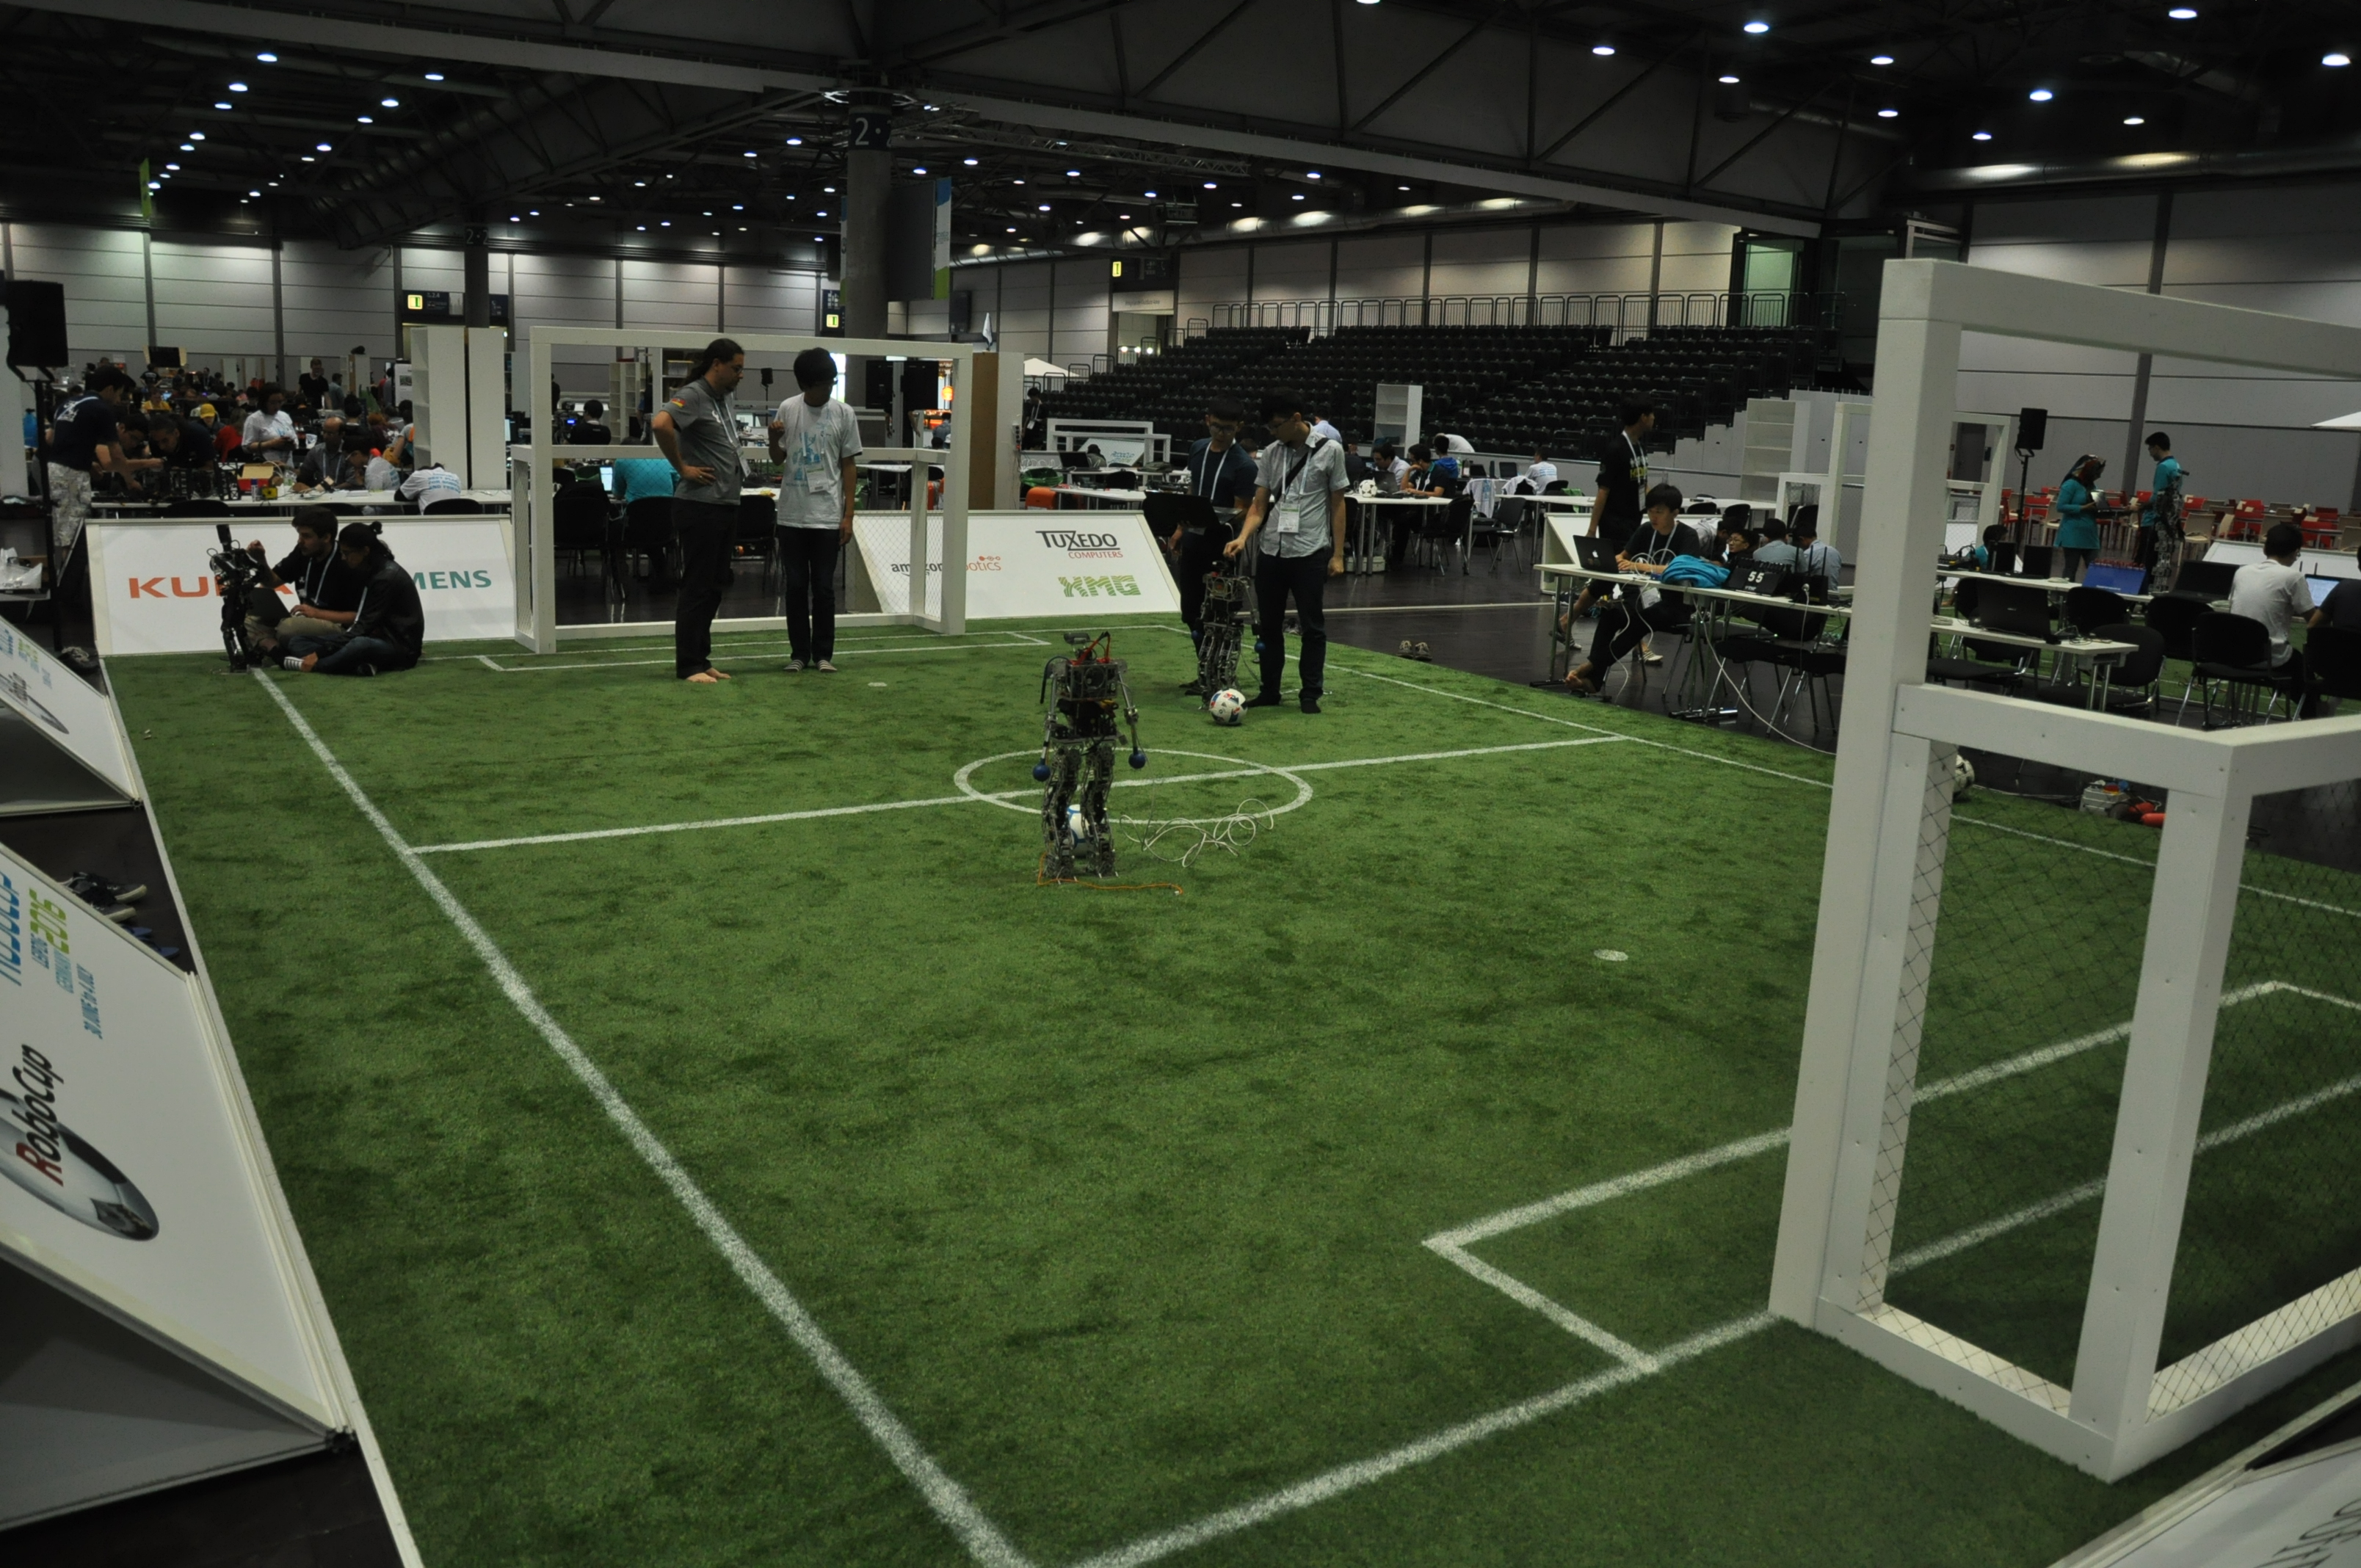
\includegraphics[width=7.5cm]{images/robocup_soccer}
        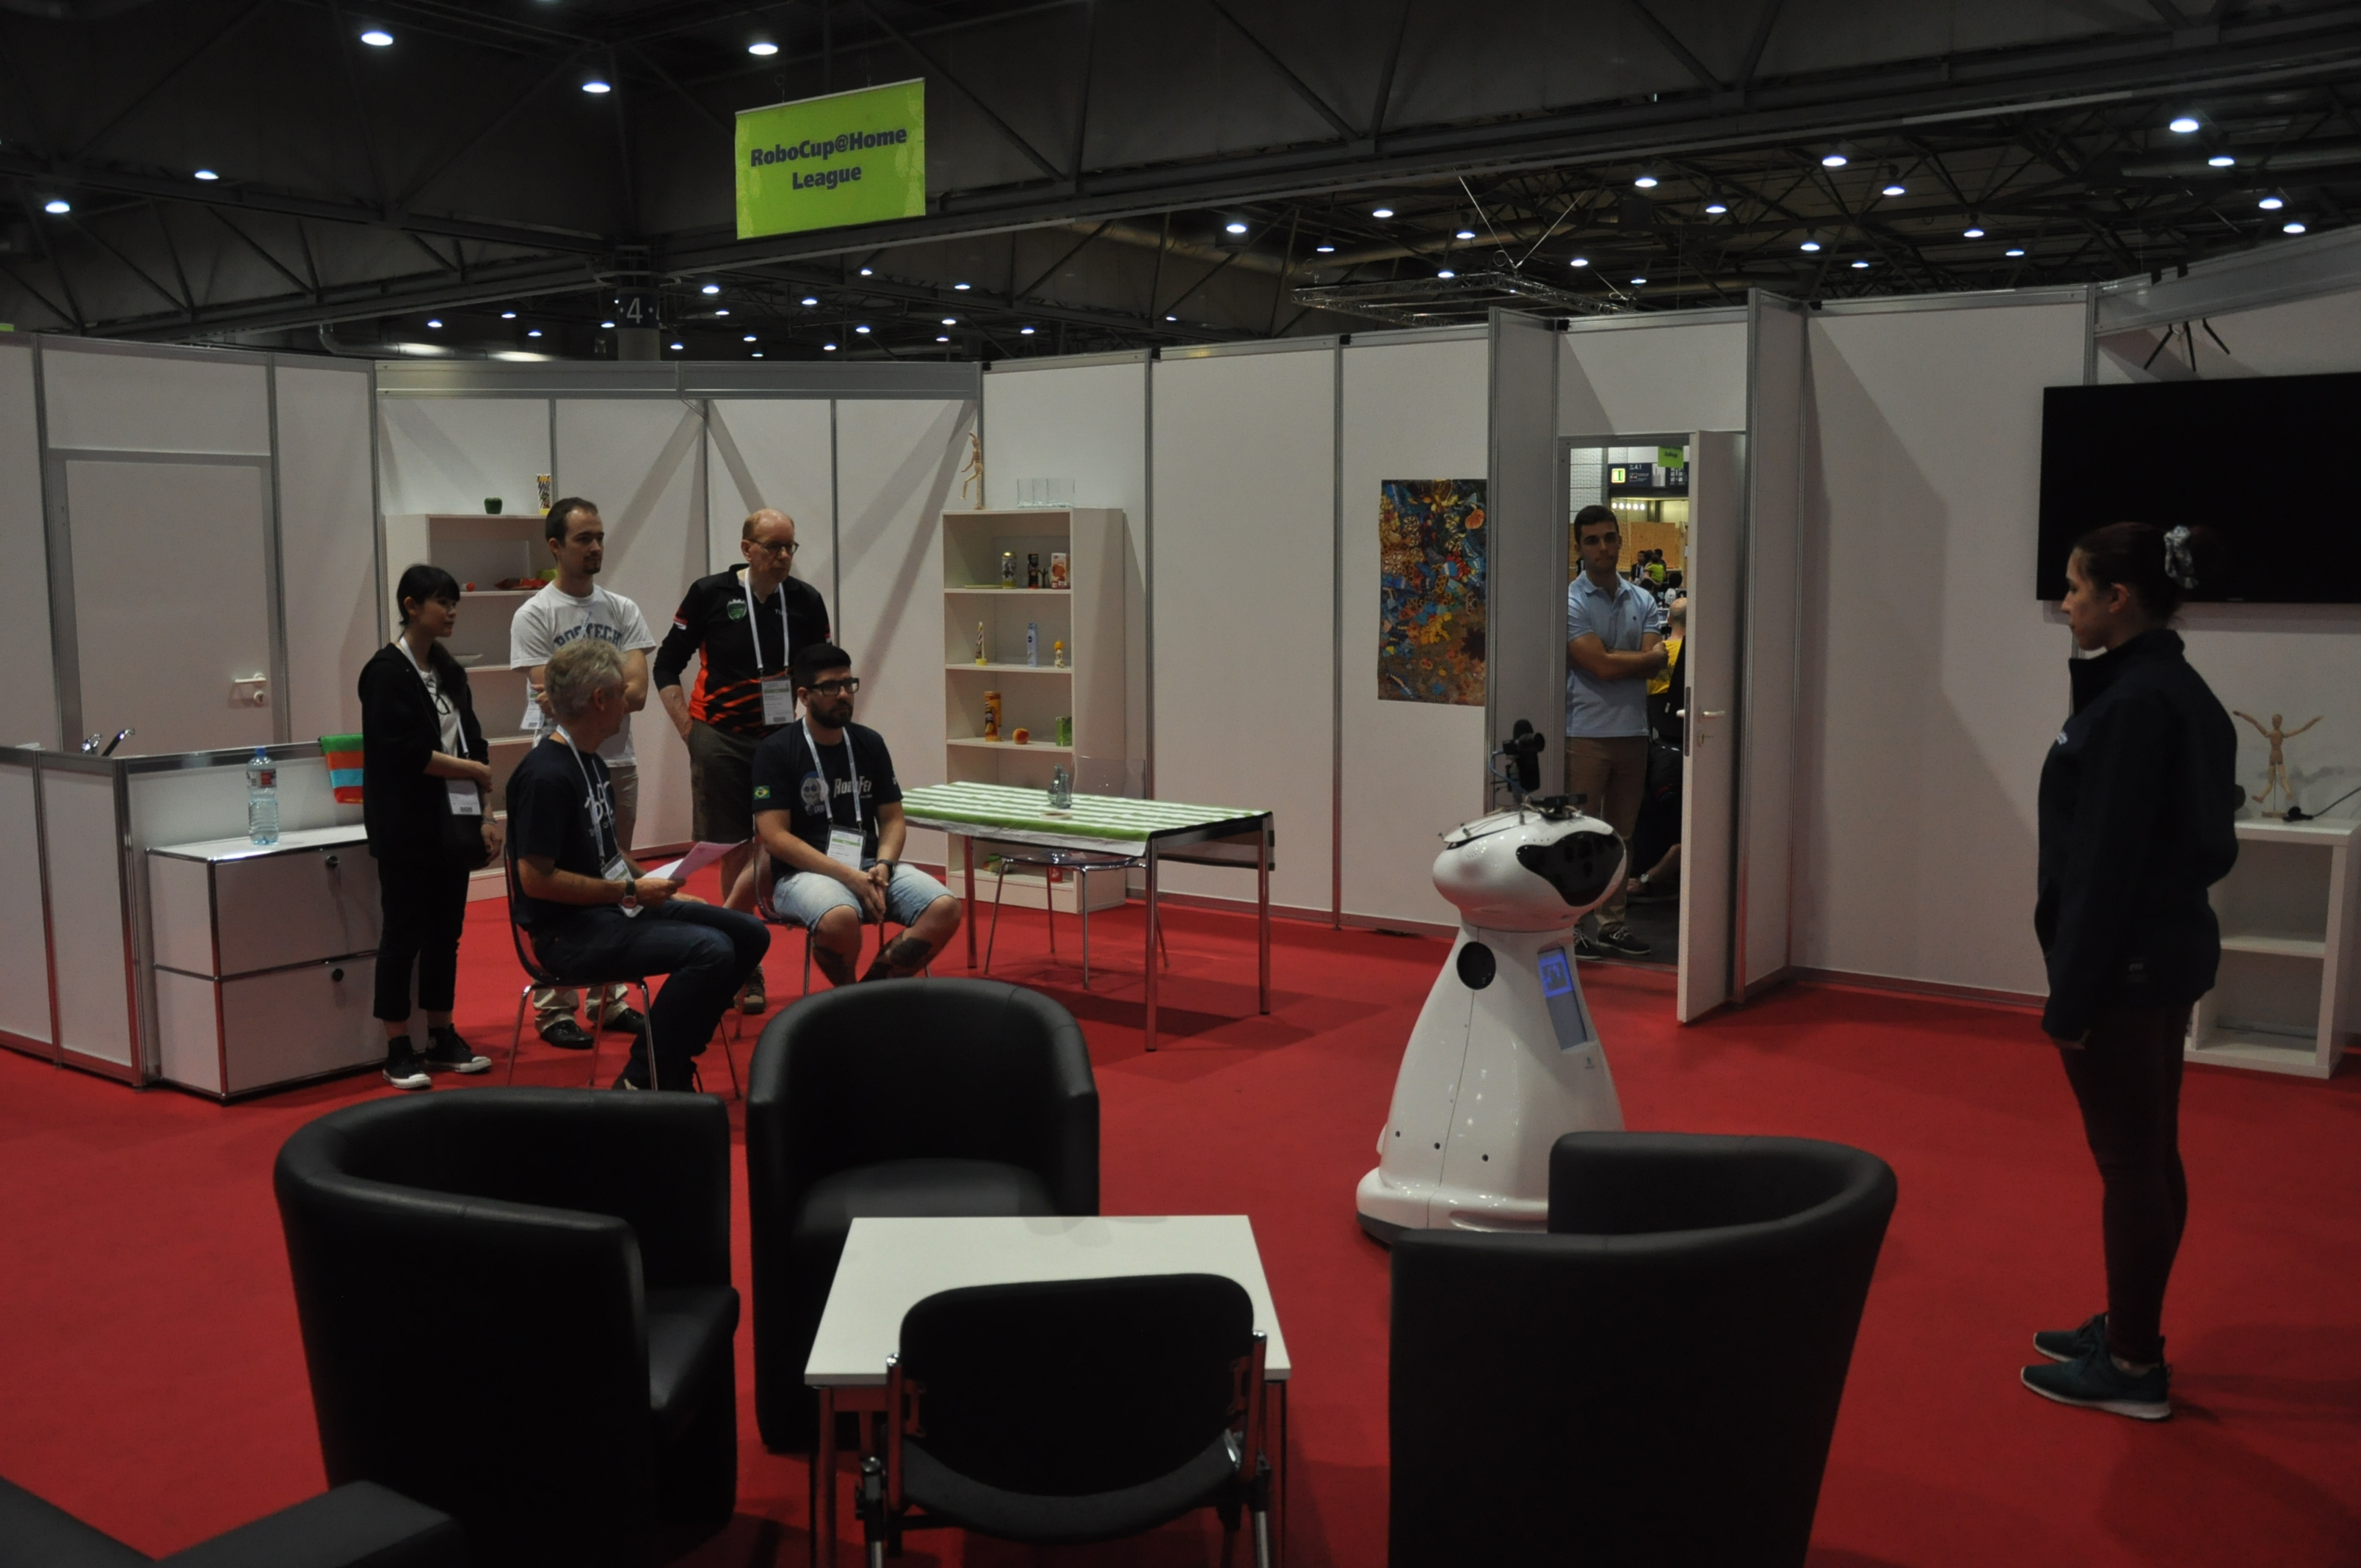
\includegraphics[width=7.5cm]{images/robocup_athome}
        \caption{On the left, it is shown a match between two teams in the
        human size robot soccer league. On the right, it is shown a run of the
        Robocup@Home tournament. These events occurred in Leipzig, 2016.}
        \label{fig:robocup_imgs}
\end{figure}

It is in this context that Robocup@Home\footnote{For more information see
\url{http://www.robocupathome.org/}} \cite{rulebook_2016} appears (among others,
e.g., Robocup@Work, Robocup Rescue, etc.), fostering research on \glspl{DSR}
and having the main goal of developing service and assistive technologies with
relevance for future personal domestic applications. \par

During the event, a set of robot capabilities are tested on specialized
environments. Major categories include: perception, human robot
interaction, mapping, navigation under highly dynamic environments and last, but
not the least, robotic manipulation. It is interesting to note that even if
tests are specialized, it does not mean they focus on single skills.
Furthermore, all these tests feature scenarios where the robot has to
use most of its capabilities in order to successfully accomplish the provided
tasks. Yet, even if the robot has the majority of these systems working
properly, he still has to reason what to do with them. For this reason, task
planning is absolutely necessary as a coordination mechanism to successfully
complete goals on these environments. \par

Even though most of this modules have matured to a point that render them
usable on non controlled environments, like robotics competitions, the same
cannot be said to the area of task planning. Most of the teams still rely
exclusively on state machines in order to provide basic reasoning to the robot.
The reasons for using state machines (e.g., SMACH\footnote{Find more about it on
\url{http://wiki.ros.org/smach}}) on these type of domains, in spite of a fully
fledged task planner, can be reduced to three factors:
\begin{itemize}
  \item Easy to structure and design;
  \item \textit{Batteries Included}, as integrated debug and monitoring tools
  are provided out of the box, making them reliable.
  \item Tasks are structured in a way that makes planning seem like an
  overengineered solution to a specific problem.
\end{itemize}

However, this approach has several problems:
\begin{itemize}
  \item Scaling to real world problems can be difficult, as state machines
  become increasingly complicated and hard to understand as the number of
  possible transitions increase;
  \item There is not a natural way to handle uncertainty coming from actions or
  observations and when they are adapted to do that, the resulting state machine
  appears hammered to solve a specific problem;
  \item Real world does not have a structured nature, rendering state machines
  incapable to acutely represent it.
\end{itemize}

For the reasons above, planning appears as an alternative to control the robot
behavior with the hope that it increases its autonomy. Furthermore, \gls{DT}
provides the basic mathematical framework in order to solve these
planning problems, with or without uncertainty on its domains, capable of
maximizing reward signals over time and/or completing goals. Applying this
knowledge into robotics, the domestic environment can be modeled as a
\gls{MDP}, taking into account the uncertainty on agent's action effects and
rewards given for reaching some state. With this framework, the agent can
decide at any time which action it should take in order to maximize this reward.
\par

Other rather important detail is that these \glspl{DSR} often face several
limitations on the actions they must perform and how they perceive the
surrounding environment. Nevertheless, there are multiple ways to overcome these
limitations, ranging from better sensors and actuators, to agents that
seek help from other agents to reach their goals. However, the first solution is
not always feasible: the robot could not withstand more weight; there is not a
sensor precise enough for the application ; or more commonly, the budget does not
accommodate any extra hardware/software to be integrated. Whereas the latter 
can be a cheaper and simpler solution for coping with these constraints.
Under these circumstances, the robot agent should try to do most of the actions
by himself, keeping its autonomy, but should ask for help whenever the success
rate for a specific action is too low and the cost for asking human cooperation
is bearable. This is an example of \gls{SA}, where the robot has to take on
tasks from people on the domestic environment, but can also ask for their help
whenever it is necessary.\par

In general, the help that these robotic agents can receive is not restricted to
physical actions, like grabbing a cup and giving it back to the robot, for
example. Therefore, a human agent can also help the robot in many other ways,
like giving him a better estimate of his position, giving him a preferable path
to cross if there is some temporary physical restriction or by telling where is
the object he is is looking for. Most of these pains are easily solved by these
human agents, wandering around on these environments.\par

All things considered, by formalizing and solving this problem, the taken
approach can be generalized to handle other kinds of domains where there is
uncertainty in the world model and rewards for executing some action along with
other human agents in the environment.

\section{Problem Description}

All things considered, the main topic of this dissertation concerns the effort
from SocRob@Home team\footnote{\url{http://socrob.isr.ist.utl.pt/}} to provide
action reasoning on domestic environments (namely on the ISRoboNet testbed)
to the Mbot robot. SocRob@Home is part of SocRob project at \textit{Institute 
for Systems and Robotics}, responsible for research in the areas of mobile service 
robots in multiple domains of interest, like domestic and healthcare facilities. During
research duties, the developed technologies are benchmarked on robotic competitions
among other highly reputable teams across the world.

\begin{figure}[H]
    \centering
        
\includegraphics[scale=0.5]{images/socrob_home_logo}
        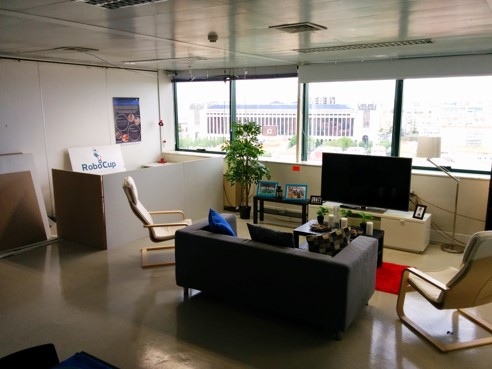
\includegraphics[scale=0.8]{images/testbed}
        \caption{SocRob@Home team logo and ISRoboNet@Home Testbed.}
        \label{fig:socrobhome}
\end{figure}

\subsection{Problem Statement}

Taking into account all tasks the mobile robot must complete in domestic
scenarios and the existing uncertainty on outcomes of agent's actions (may them 
be its own actions or its requests for help), this
agent should make decisions that lead it to the best outcome possible, given
any possible situation achieved, on a countable sequence of steps. So the 
objective is to integrate a planner which can attain that, into a real robot.
The planner should be able to deal with discrete and continuous action effects 
while being able to cope with new information given to it (i.e. new objects or people
in the environment from one step to another).

\subsection{Approach}

In order to achieve this behavior, the agent should have a world model of the
domestic environment\footnote{This is not absolutely necessary if the problem is
solved using other methods from \gls{DT} like reinforcement learning, for example.},
including possible states and respective rewards along with actions available to
be performed by the robot. In fact, to model these domains in an efficient
manner, there are the following tools capable of handling uncertainty on their
domains:
\begin{itemize}
\item \gls{MDP} or \gls{POMDP}: the classical approach, following well known mathematical
procedures.
\item \gls{DBN}: by drawing the world model, along with the correspondent
probability distributions, on a classical structure of probability
theory\footnote{OpenMarkov is a common tool used for this purpose. See more at
\url{http://www.openmarkov.org/}}.
\item \gls{PDL}: Using declarative languages such as \gls{PPDDL}
\cite{younes2004ppddl1} or \gls{RDDL} \cite{Sanner_RDDL} to describe the world
model, according to a set of syntax and semantic rules. They are normally used
in competitions like \gls{ICAPS-IPC}\footnote{Discover more about these type of
competitions here:
\url{http://www.icaps-conference.org/index.php/Main/Competitions}},
decoupling the planner from the language used to describe the world model.
\item \glspl{PLPL}: the world model is formalized on a completely capable
logical programming language and the solver comes as a builtin of the
programming language.
\end{itemize}

For the tools listed above, it was choosen the latter as a building block of
the framework, namely the \gls{HYPE} planner \cite{nitti2015planning}. As a result,
one of the goals of this dissertation is to validate the usage of this
framework on real domestic environments. The model must incorporate the
possibility that the robot interacts with humans and the other way around,
whenever is necessary, giving mutual cooperation capabilities to these agents.
To emphasize this requirement, it must be capable to describe advanced
behaviors, particularly \gls{SA} as an alternative to complete tasks on the
domestic environment.
In conclusion, this model must also represent the chance that execution of an
action will lead to many possible different effects, i.e. the model should
represent uncertainty on these actions that the robot can perform.

\section{Work Outline}

In summary, the present dissertation is structured as follows:
\begin{itemize}
  \item On the second chapter, it is explained all the
  basis needed to understand how the proposed framework has been put together.
  Starting from logical programming and finding its roots on first order logic,
  through newer probabilistic logic programming paradigms and its respective
  extensions.
  Further along the line, it is made a brief introduction to \glspl{MDP},
  domain modeling tools and finally planning, following a discussion on the
  classical solving methods and newer alternatives coming from \gls{ICAPS-IPC}.
  On the end of this topic, it is discussed introduced \gls{HYPE} planner as it is the
  building block of the proposed approach.
  It is a great idea to view and more importantly, understand figure
  \ref{fig:diagramofthesis} to get the big picture of how these pieces fit
  together.
  \begin{figure}[H]
      \centering
          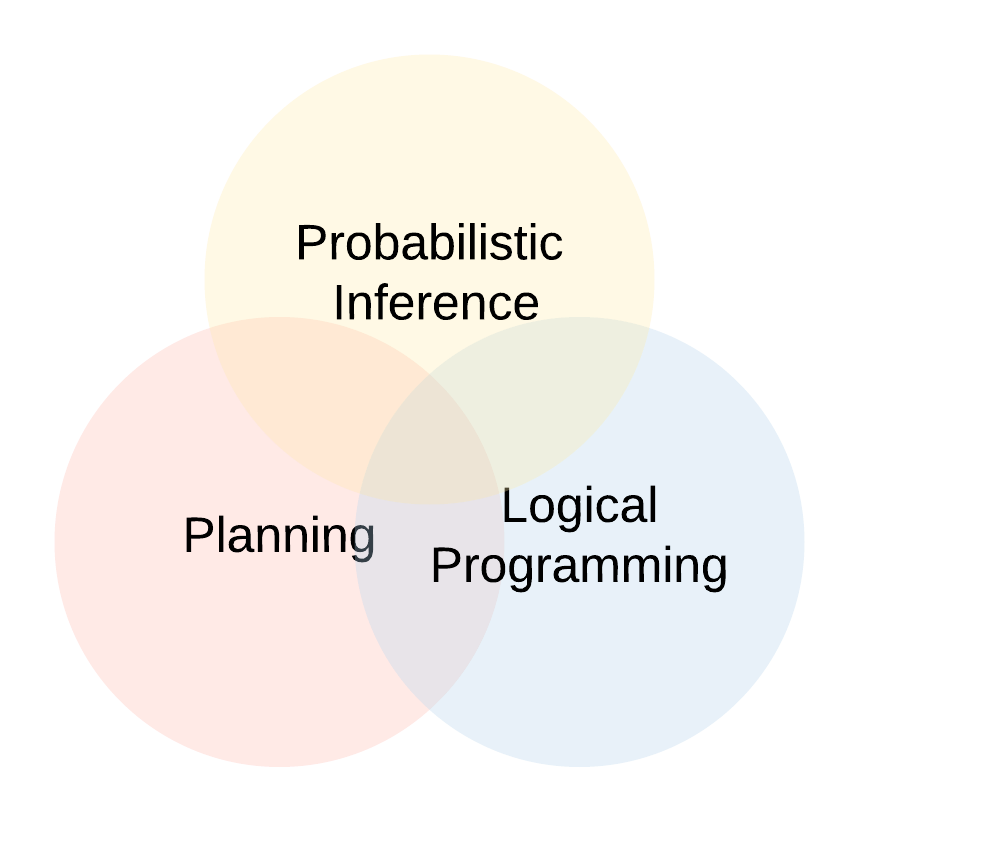
\includegraphics[scale=0.25]{images/venn}
          \caption{The \textit{Venn diagram} above shows 3 different areas of
          interest that are encapsulated by the proposed framework: Logical
          Programming, Probabilistic Inference and Planning. The theoretical
          ground for this dissertation is logical programming. An example of a
          logical programming language is Prolog, for instance. Following the
          same line of thought, probabilistic inference gives mathematical tools
          to discover the likelihood of a particular event. Planning uses
          Decision Theoretic tools in order to find which decision should be
          made on each step of a process.}
          \label{fig:diagramofthesis}
  \end{figure}
  Consequently, it is explained what is the
  concept of Symbiotic Autonomy as well as the related work on this area.
  \item Then, on the third chapter, it is discussed the implementation of the
  framework. Afterwards, the domain used on this task is explained, that is both
  robot and human agents acting in the scene and the testbed, simulating a
  domestic environment. Finally, the planning framework architecture is
  explained, as well as each one of its procedures.
  \item The fourth chapter is about the evalutation of the pipeline on simulation 
  and in the real world. Starting from a description of the robot, in terms of its relevant
  hardware and software modules and ending in the testbed. Results from the planning framework are collected,
  not only from simulation scenarios but also from the real test scenario with
  real agents. 
  \item Then, there is also a discussion about the results obtained. In
  particular, the following questions are answered:\textit{"Does the
  framework produce meaningful results?"}; \textit{"Is the framework usable in real
  environments?"}.
  Not only are these questions answered, but also some remarks are made about
  the lessons learned.

  \item In the last chapter, a conclusion is made about what was achieved in this thesis.
\end{itemize}
